%  LaTeX support: latex@mdpi.com 
%  For support, please attach all files needed for compiling as well as the log file, and specify your operating system, LaTeX version, and LaTeX editor.

%=================================================================
\documentclass[mathematics,review,submit,moreauthors,pdftex]{Definitions/mdpi} 

% For posting an early version of this manuscript as a preprint, you may use "preprints" as the journal and change "submit" to "accept". The document class line would be, e.g., \documentclass[preprints,article,accept,moreauthors,pdftex]{mdpi}. This is especially recommended for submission to arXiv, where line numbers should be removed before posting. For preprints.org, the editorial staff will make this change immediately prior to posting.

%--------------------
% Class Options:
%--------------------
%----------
% journal
%----------
% Choose between the following MDPI journals:
% acoustics, actuators, addictions, admsci, adolescents, aerospace, agriculture, agriengineering, agronomy, ai, algorithms, allergies, analytica, animals, antibiotics, antibodies, antioxidants, appliedchem, applmech, applmicrobiol, applnano, applsci, arts, asi, atmosphere, atoms, audiolres, automation, axioms, batteries, bdcc, behavsci, beverages, biochem, bioengineering, biologics, biology, biomechanics, biomedicines, biomedinformatics, biomimetics, biomolecules, biophysica, biosensors, biotech, birds, bloods, brainsci, buildings, businesses, cancers, carbon, cardiogenetics, catalysts, cells, ceramics, challenges, chemengineering, chemistry, chemosensors, chemproc, children, civileng, cleantechnol, climate, clinpract, clockssleep, cmd, coatings, colloids, compounds, computation, computers, condensedmatter, conservation, constrmater, cosmetics, crops, cryptography, crystals, curroncol, cyber, dairy, data, dentistry, dermato, dermatopathology, designs, diabetology, diagnostics, digital, disabilities, diseases, diversity, dna, drones, dynamics, earth, ebj, ecologies, econometrics, economies, education, ejihpe, electricity, electrochem, electronicmat, electronics, encyclopedia, endocrines, energies, eng, engproc, entropy, environments, environsciproc, epidemiologia, epigenomes, fermentation, fibers, fire, fishes, fluids, foods, forecasting, forensicsci, forests, fractalfract, fuels, futureinternet, futuretransp, futurepharmacol, futurephys, galaxies, games, gases, gastroent, gastrointestdisord, gels, genealogy, genes, geographies, geohazards, geomatics, geosciences, geotechnics, geriatrics, hazardousmatters, healthcare, hearts, hemato, heritage, highthroughput, histories, horticulturae, humanities, hydrogen, hydrology, hygiene, idr, ijerph, ijfs, ijgi, ijms, ijns, ijtm, ijtpp, immuno, informatics, information, infrastructures, inorganics, insects, instruments, inventions, iot, j, jcdd, jcm, jcp, jcs, jdb, jfb, jfmk, jimaging, jintelligence, jlpea, jmmp, jmp, jmse, jne, jnt, jof, joitmc, jor, journalmedia, jox, jpm, jrfm, jsan, jtaer, jzbg, kidney, land, languages, laws, life, liquids, literature, livers, logistics, lubricants, machines, macromol, magnetism, magnetochemistry, make, marinedrugs, materials, materproc, mathematics, mca, measurements, medicina, medicines, medsci, membranes, metabolites, metals, metrology, micro, microarrays, microbiolres, micromachines, microorganisms, minerals, mining, modelling, molbank, molecules, mps, mti, nanoenergyadv, nanomanufacturing, nanomaterials, ncrna, network, neuroglia, neurolint, neurosci, nitrogen, notspecified, nri, nursrep, nutrients, obesities, oceans, ohbm, onco, oncopathology, optics, oral, organics, osteology, oxygen, parasites, parasitologia, particles, pathogens, pathophysiology, pediatrrep, pharmaceuticals, pharmaceutics, pharmacy, philosophies, photochem, photonics, physchem, physics, physiolsci, plants, plasma, pollutants, polymers, polysaccharides, proceedings, processes, prosthesis, proteomes, psych, psychiatryint, publications, quantumrep, quaternary, qubs, radiation, reactions, recycling, regeneration, religions, remotesensing, reports, reprodmed, resources, risks, robotics, safety, sci, scipharm, sensors, separations, sexes, signals, sinusitis, smartcities, sna, societies, socsci, soilsystems, solids, sports, standards, stats, stresses, surfaces, surgeries, suschem, sustainability, symmetry, systems, taxonomy, technologies, telecom, textiles, thermo, tourismhosp, toxics, toxins, transplantology, traumas, tropicalmed, universe, urbansci, uro, vaccines, vehicles, vetsci, vibration, viruses, vision, water, wevj, women, world 

%---------
% article
%---------
% The default type of manuscript is "article", but can be replaced by: 
% abstract, addendum, article, book, bookreview, briefreport, casereport, comment, commentary, communication, conferenceproceedings, correction, conferencereport, entry, expressionofconcern, extendedabstract, datadescriptor, editorial, essay, erratum, hypothesis, interestingimage, obituary, opinion, projectreport, reply, retraction, review, perspective, protocol, shortnote, studyprotocol, systematicreview, supfile, technicalnote, viewpoint, guidelines, registeredreport, tutorial
% supfile = supplementary materials

%----------
% submit
%----------
% The class option "submit" will be changed to "accept" by the Editorial Office when the paper is accepted. This will only make changes to the frontpage (e.g., the logo of the journal will get visible), the headings, and the copyright information. Also, line numbering will be removed. Journal info and pagination for accepted papers will also be assigned by the Editorial Office.

%------------------
% moreauthors
%------------------
% If there is only one author the class option oneauthor should be used. Otherwise use the class option moreauthors.

%---------
% pdftex
%---------
% The option pdftex is for use with pdfLaTeX. If eps figures are used, remove the option pdftex and use LaTeX and dvi2pdf.

%=================================================================
% MDPI internal commands
\firstpage{1} 
\makeatletter 
\setcounter{page}{\@firstpage} 
\makeatother
\pubvolume{1}
\issuenum{1}
\articlenumber{0}
\pubyear{2021}
\copyrightyear{2020}
\externaleditor{Academic Editor: } % For journal Automation, please change Academic Editor to "Communicated by"
\datereceived{} 
\dateaccepted{} 
\datepublished{} 
\hreflink{https://doi.org/} % If needed use \linebreak
%------------------------------------------------------------------
% The following line should be uncommented if the LaTeX file is uploaded to arXiv.org
%\pdfoutput=1

%=================================================================
% Add packages and commands here. The following packages are loaded in our class file: fontenc, inputenc, calc, indentfirst, fancyhdr, graphicx, epstopdf, lastpage, ifthen, lineno, float, amsmath, setspace, enumitem, mathpazo, booktabs, titlesec, etoolbox, tabto, xcolor, soul, multirow, microtype, tikz, totcount, changepage, paracol, attrib, upgreek, cleveref, amsthm, hyphenat, natbib, hyperref, footmisc, url, geometry, newfloat, caption

\usepackage{tabulary}

%=================================================================
%% Please use the following mathematics environments: Theorem, Lemma, Corollary, Proposition, Characterization, Property, Problem, Example, ExamplesandDefinitions, Hypothesis, Remark, Definition, Notation, Assumption
%% For proofs, please use the proof environment (the amsthm package is loaded by the MDPI class).

%=================================================================
% Full title of the paper (Capitalized)
\Title{A Survey on Software Defect Prediction Using Deep Learning}

% MDPI internal command: Title for citation in the left column
\TitleCitation{A Survey on Software Defect Prediction Using Deep Learning}

% Author Orchid ID: enter ID or remove command
\newcommand{\orcidauthorA}{0000-0002-4462-5817} % Elena N. Akimova Add \orcidA{} behind the author's name
\newcommand{\orcidauthorB}{0000-0002-5565-0583} % Vladimir E. Misilov Add \orcidB{} behind the author's name
\newcommand{\orcidauthorC}{0000-0002-0037-2352} % Anton V. Konygin Add \orcidC{} behind the author's name
%\newcommand{\orcidauthorD}{0000-0000-0000-000X} % Add \orcidD{} behind the author's name
%\newcommand{\orcidauthorE}{0000-0000-0000-000X} % Add \orcidE{} behind the author's name
%\newcommand{\orcidauthorF}{0000-0000-0000-000X} % Add \orcidF{} behind the author's name

% Authors, for the paper (add full first names)
\Author{Elena~N.~Akimova $^{1,2,}*$\orcidA{}, Alexander~Yu.~Bersenev $^{1,2}$, Artem~A.~Deikov $^{1,2}$, Konstantin~S.~Kobylkin $^{1,2}$, Anton~V.~Konygin $^{1}$\orcidC{}, Ilya~P.~Mezentsev $^{1,2}$, and Vladimir~E.~Misilov $^{1,2}\orcidB{}$}

% MDPI internal command: Authors, for metadata in PDF
\AuthorNames{Elena N. Akimova, Alexander Yu. Bersenev, Artem A. Deikov, Konstantin S. Kobylkin, Anton V. Konygin, Ilya P. Mezentsev, and Vladimir E. Misilov}

% MDPI internal command: Authors, for citation in the left column
\AuthorCitation{Akimova,~E.~N.; Bersenev,~A.~Yu.; Deikov,~A.~A.; Kobylkin,~K.~S.; Konygin,~A.~V.; Mezentsev,~I.~P.; Misilov,~V.~E.}
% If this is a Chicago style journal: Lastname, Firstname, Firstname Lastname, and Firstname Lastname.

% Affiliations / Addresses (Add [1] after \address if there is only one affiliation.)
\address{%
$^{1}$ \quad Krasovskii Institute of Mathematics and Mechanics, Ural Branch of RAS, S.~Kovalevskaya Street 16, Ekaterinburg, Russia; Alexander.Bersenev@urfu.ru (A.Yu.B.); hx0day@hackerdom.ru (A.A.D); kobylkinks@gmail.com (K.S.K); konygin@imm.uran.ru (A.V.K.); ilyamezentcev@gmail.com (I.P.M); v.e.misilov@urfu.ru (V.E.M.)\\
$^{2}$ \quad Ural Federal University, Mira Street 19, Ekaterinburg, Russia;}

% Contact information of the corresponding author
\corres{Correspondence: aen15@yandex.ru}

% Current address and/or shared authorship
%\firstnote{Current address: Affiliation 3} 
%\secondnote{These authors contributed equally to this work.}
% The commands \thirdnote{} till \eighthnote{} are available for further notes

%\simplesumm{} % Simple summary

%\conference{} % An extended version of a conference paper

% Abstract (Do not insert blank lines, i.e. \\) 
\abstract{Defect prediction is one of key challenges in software development and programming language research for improving software quality and reliability. 
The problem in this area is to properly identify the defective source code with high accuracy.
Developing fault prediction model is a challenging problem, and many approaches have been proposed through the history. 
The recent breakthrough in machine learning technologies, especially, the development of deep learning techniques, led to the fact that many problems can be solved by these methods.
Our survey focuses on the deep learning techniques for defect prediction. We analyse the recent works on the topic, study the methods for automatical learning of the semantic and structural features from the code, discuss the open problems, and present the recent trends in the field.}

% Keywords
\keyword{Defect prediction; Anomaly detection; Program analysis; Code understanding; Neural Networks; Deep Learning} 

% The fields PACS, MSC, and JEL may be left empty or commented out if not applicable
%\PACS{J0101}
\MSC{68N30; 68T07}
%\JEL{}

%%%%%%%%%%%%%%%%%%%%%%%%%%%%%%%%%%%%%%%%%%
% Only for the journal Diversity
%\LSID{\url{http://}}

%%%%%%%%%%%%%%%%%%%%%%%%%%%%%%%%%%%%%%%%%%
% Only for the journal Applied Sciences:
%\featuredapplication{Authors are encouraged to provide a concise description of the specific application or a potential application of the work. This section is not mandatory.}
%%%%%%%%%%%%%%%%%%%%%%%%%%%%%%%%%%%%%%%%%%

%%%%%%%%%%%%%%%%%%%%%%%%%%%%%%%%%%%%%%%%%%
% Only for the journal Data:
%\dataset{DOI number or link to the deposited data set in cases where the data set is published or set to be published separately. If the data set is submitted and will be published as a supplement to this paper in the journal Data, this field will be filled by the editors of the journal. In this case, please make sure to submit the data set as a supplement when entering your manuscript into our manuscript editorial system.}

%\datasetlicense{license under which the data set is made available (CC0, CC-BY, CC-BY-SA, CC-BY-NC, etc.)}

%%%%%%%%%%%%%%%%%%%%%%%%%%%%%%%%%%%%%%%%%%
% Only for the journal Toxins
%\keycontribution{The breakthroughs or highlights of the manuscript. Authors can write one or two sentences to describe the most important part of the paper.}

%%%%%%%%%%%%%%%%%%%%%%%%%%%%%%%%%%%%%%%%%%
% Only for the journal Encyclopedia
%\encyclopediadef{Instead of the abstract}
%\entrylink{The Link to this entry published on the encyclopedia platform.}
%%%%%%%%%%%%%%%%%%%%%%%%%%%%%%%%%%%%%%%%%%
\begin{document}
%%%%%%%%%%%%%%%%%%%%%%%%%%%%%%%%%%%%%%%%%%
%\setcounter{section}{-1} %% Remove this when starting to work on the template.

\section{Introduction}\label{sec_1}

According to the IEEE Standard Classification for Software Anomalies~\cite{ieee_standard}, a software defect is ``an imperfection or deficiency in a work product where that work product does not meet its requirements or specifications and needs to be either repaired or replaced''.

Software defects can cause different problems.
Common ways for finding the software defects are the manual testing and code review. The main drawback of these methods is that they are quite expensive in terms of time and effort. The automatic approaches to the Software Defect Prediction (SDP) would allow one to recude the costs and improve quality of the software projects.

Thus, Software Defect Prediction is an important problem in the fields of the software engineering and programming language research.
The task is to identify the defective code with high accuracy (in terms of the precision and recall).

The development and breakthrough of machine learning led to the fact that many tasks can be solved by the these methods.

Recent advances in the fields of artificial neural networks and machine learning, as well as, the increasing power of the modern computers (such as supercomputers based on GPUs with AI accelerating modules) allowed the new concepts, such as deep learning, to emerge.
The main idea is that an artificial neural network with multiple layers is capable to progressively extract the higher-level features from the original data to solve complex problems.

For the problem of software defect prediction, the researchers have proposed the re\-pre\-sen\-ta\-tion-learning algorithms to learn semantic representations of programs automatically and use this representation to identify the defect-prone code. Using these implicit features shows better results then the previous approaches based on the explicit features, such as the code metrics~\cite{WangEtAl2016}. 

The software defect prediction is a rapidly developing field, and the state-of-the-art surveys on the topic~\cite{OmriSinz2020Survey,yang2020survey,ShenChen2020Survey} do not sufficiently cover the recent works describing the cutting-edge techniques. For example, recent advances in the related fields of Natural Language Processing (NLP) provided the new powerful tools such as Transformer language models. These techniques were later successfully applied to the software engineering tasks. 

The goal of our survey is to describe these latest achievements taking into account the newest primary studies published in 2019--2021. We hope that this survey can be useful for researchers and practitioners in the software defect prediction, code understanding, and other related fields.

Some semantic defects are hard to find using only source code. For example, in~\cite{BryksinEtAl2020}, the bytecode of Kotlin programs is processed to detect the so called compiler-induced anomalies, which arise only in the compiled bytecode. Another example is presented in work~\cite{PhanNguyen2017} where to expose the program behavior, the 
assembly code (generated from the C source code by the compiler) is used to learn the defect features.

Nevertheless, the source code remains the main source of data for the defect prediction. 
In this survey, our main interest lies in techniques devoted to analyzing the source code. Usually, the process of developing the model for the defect prediction consists of the following steps (see Fig.~\ref{fig1}):
\begin{enumerate}
\item Prepare the dataset by collecting the source code samples from repositories of the software projects (or choose the suitable existing dataset).
\item Extract features from the source code.
\item Train the model using the train dataset.
\item Test the model using the test dataset and assess the performance using the quality metrics.
\end{enumerate}

\begin{figure}[ht] %s state preferences regarding figure placement here
% use to correct figure counter if necessary
%\renewcommand{\thefigure}{2}
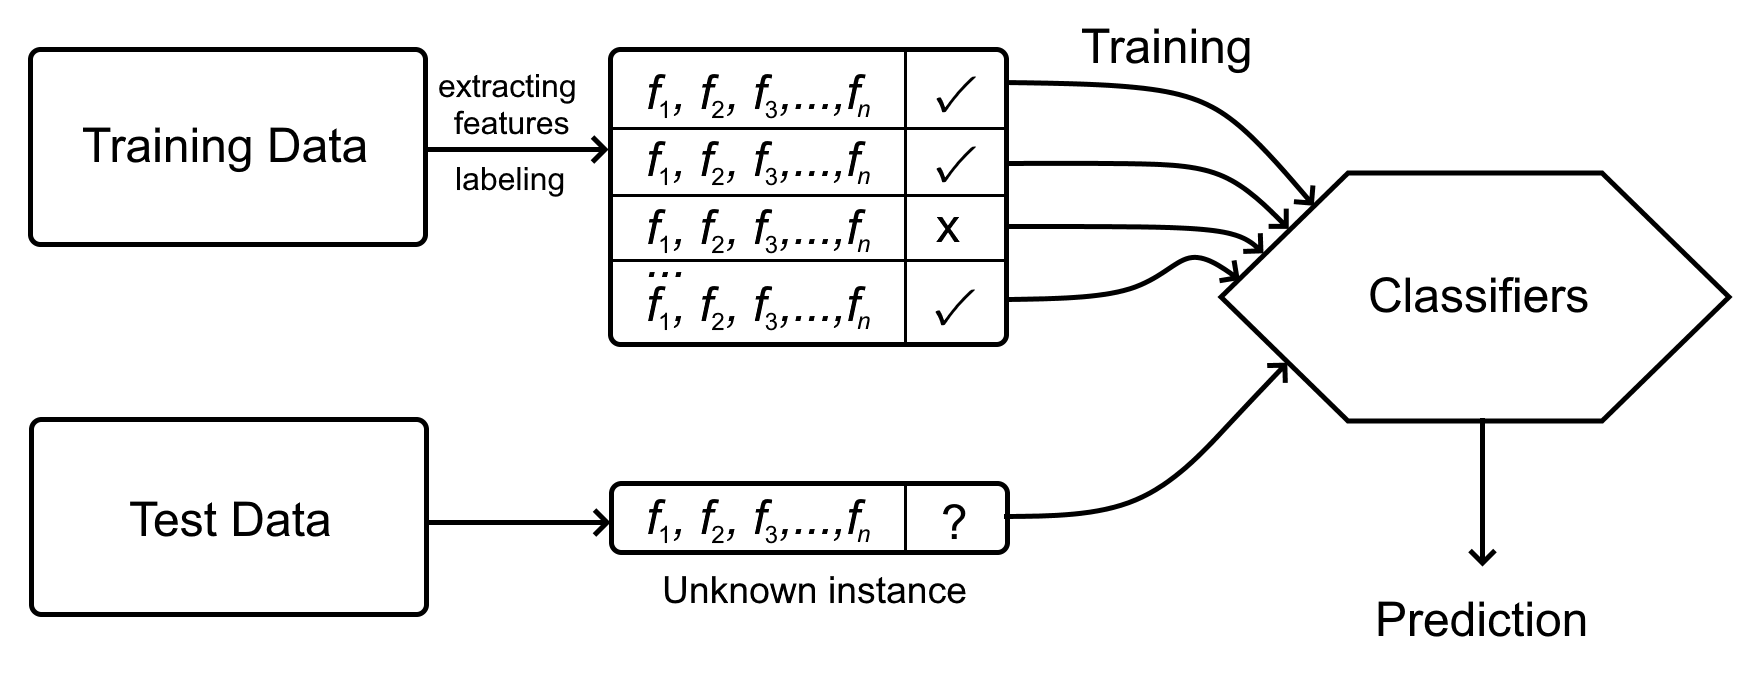
\includegraphics[width=11.5 cm]{f1.png}
\caption{Scheme of the the process of constructing the defect prediction model.}
\label{fig1} % \label works only AFTER \caption within figure environment
\end{figure}

The survey is structured as follows. Section~\ref{sec_2} briefly describes the methodology of our survey. Section~\ref{sec_3} presents the overview on the various deep learning techniques applied to the defect prediction. In Section~\ref{sec_4}, we outline the main difficulties of the problem. Section~\ref{sec_5} presents the study of the latest trends in the techniques and methods for defect prediction. Section~\ref{sec_6} concludes the study and offers our vision on the future developments on the field.

%%%%%%%%%%%%%%%%%%%%%%%%%%%%%%%%%%%%%%%%%%
\section{Methodology}\label{sec_2}

We reviewed the primary studies on the subject. In this section, we present details of our methodology.

\subsection{Research Questions}

To summarize the work of our survey, let us formulate the following research questions:

\begin{itemize}
\item RQ1. What deep learning techniques have been applied to the software defect prediction?
\item RQ2. What are the key factors contributing to difficulty of the problem?
\item RQ3. What are the trends in the primary studies on the use of deep learning for the software defect prediction?
\end{itemize}

\subsection{Literature Search and Inclusion or Exclusion Criteria}

To collect related papers, we formulated a search string for Google Scholar and Scopus combining the related keywords "software engineering", "deep learning", and "defect prediction".

To filter the papers with insufficient content and determine the paper quality, we used the following criteria:

\begin{itemize}
\item The paper must describe a technique for automatic feature extraction using deep learning and apply it to defect prediction problem
\item The paper length must not be less than 6 pages
\end{itemize}


%%%%%%%%%%%%%%%%%%%%%%%%%%%%%%%%%%%%%%%%%%
\section{RQ1. What techniques have been applied to this problem?}\label{sec_3}

In order to work with the source code, we need to have its representation.
On the one hand, this representation should be simple as a vector, since most of machine learning algorithms work with vectors.
On the other hand, the representation should contain all necessary information. 
The numerical vector representing the source code is called an ``embedding''.

There are different ways to represent the source code. Moreover, we need different granularities for different tasks, \textit{e.g.}, for code completion we need token-level embedding and for function clone detection we need function embedding. For the software defect prediction problem, various levels of granularity are used, such as sub-system, component, file/class, method, and change (see \cite{AllamanisEtAl2018,ChenMonperrus2019} for more info on various code embeddings).

One way is to create the vector from the hand crafted features.
This approach assumes that an expert invents a set of features and selects best of them, (e.g., \cite{SharminEtAl2015,DamEtAl2018}).
Usually, these features include the statistical characteristics of code, such as its size, code complexity, code churn, or process metrics.

Other way is to create the numerical vector by processing the source code.

One way to represent the code is a sequence of elements. Usually, they are code tokens or characters~\cite{MikolovEtAl2013}. The neural networks based on the sequences are usually trained to predict the subsequent element.

Another approach to build the representation of the source code is the abstract syntax trees (AST)~\cite{ZhangEtAl2019}. The nodes of the tree corresponds to the statement and operators, and the leaves represent the operands and values. The tree-based models are trained to predict the code by generating new nodes taking into account the existing tree structure. 

The most common approach to defect prediction is to use some classification algorithm to divide the source code into two categories: defect code and correct one (\textit{e.g.}~\cite{PradelSen2018}).

However, the approaches based on the hand-crafted features usually do not sufficiently capture the syntax and semantics of the source code. 
Most traditional code metrics cannot distinguish code fragments if these fragments have the same structure and complexity but implement different functionality.
For example, if we switch several lines in the code fragments, traditional features, such as the number of lines of code, number of function calls, number of tokens would remain the same (see~\cite{WangEtAl2016}). Thus, the semantic information is more important for defect prediction than these metrics.

Modern approaches are usually based on extracting the implicit structural, syntax, and semantic feature from the source code rather than using the explicit hand-crafted ones.

The most popular deep learning techniques for the software defect prediction are: Deep Belief Networks (DBN), Convolutional Neural Networks (CNN), Long Short Term Memory (LSTM), and Transformer architecture.

\subsection{Deep Belief Networks}

A Deep Belief Network~\cite{Bengio2009dbn} generative models are based on a multilevel neural network. This network contains one input layer, one output layer, and multiple hidden layers. The output layer generates a feature vector representing the data fed to the input layer. Each layer consists of the stochastic nodes. The important feature of the DBN is that the nodes are only connected to the nodes in the adjacent layers, but not to the nodes within the same layer as shown in Fig.~\ref{fig2}.

\begin{figure}[ht] %s state preferences regarding figure placement here
% use to correct figure counter if necessary
%\renewcommand{\thefigure}{2}
\centering
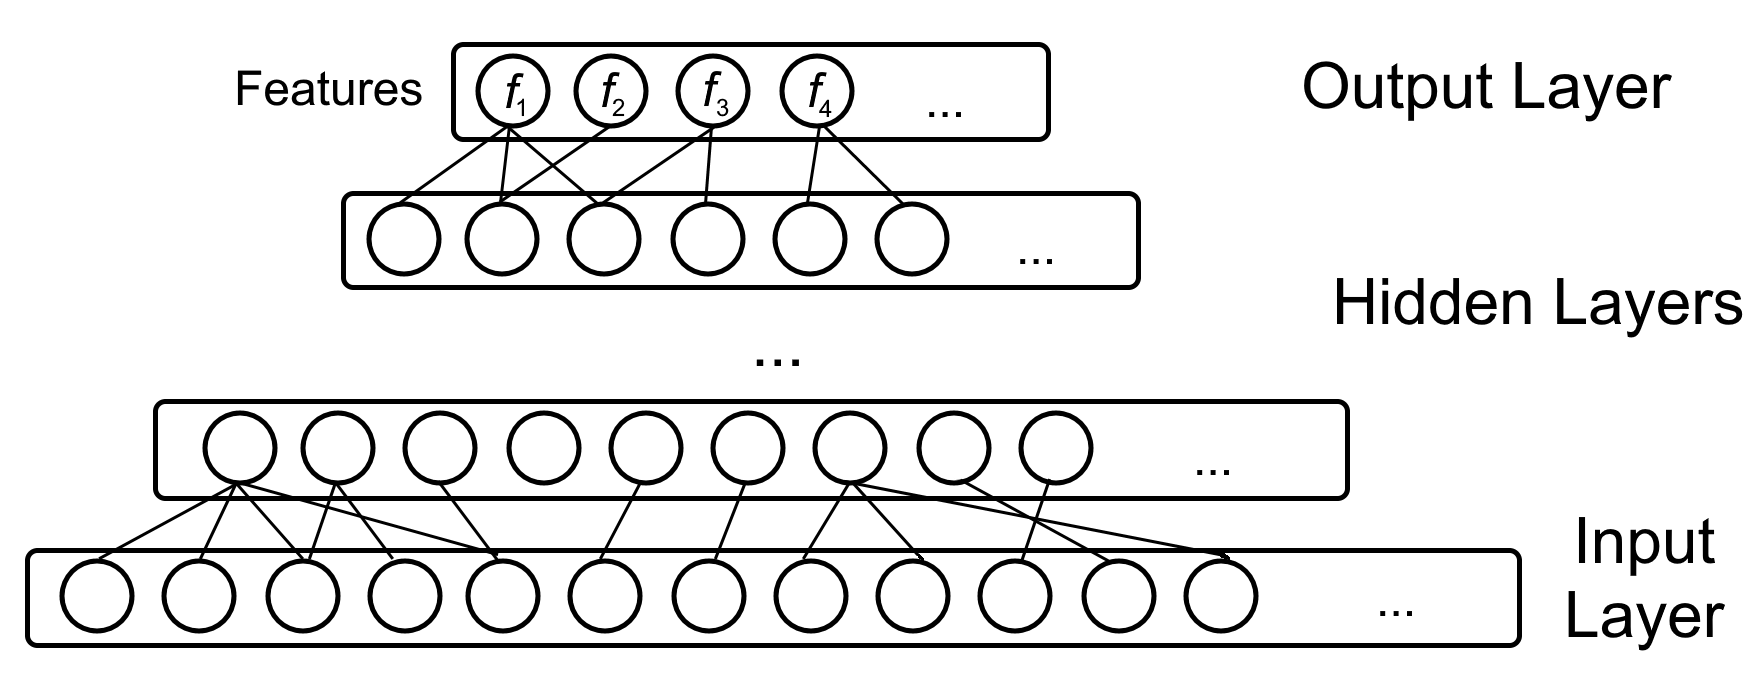
\includegraphics[width=10.5 cm]{f2.png}
\caption{Architecture of the Deep Belief Network.}
\label{fig2} % \label works only AFTER \caption within figure environment
\end{figure}

Perhaps one of the first works combining AST with the deep learning is \cite{YangEtAl2015}. The authors propose the approach for software defect prediction on changes level. 
The DBN (which is fed by the traditional code metrics) generates the new expressive features and use them in a classical machine learning classifiers. 
They extract the relations from the traditional code metrics, such as number of modified modules, directories, and files, added and deleted lines, and several features related to developer's experience. Later the authors have proposed the "TLEL" approach~\cite{YangEtAl2017} based on the decision tree and ensemble learning for classification. %In the inner layer, it combines decision tree and bagging to build the Random Forest model. In the outer layer, it uses random under-sampling to train many different Random Forest models and stacking to ensemble them once more.

The works of Wang et al.~\cite{WangEtAl2016, WangEtAl2018} also use the DBN, but in a different manner.
For predicting the defects on the basis of the code semantics, the authors have developed a DBN to automatically learn a semantic features from the source code. As the input for the network, the programs' AST and source code changes are used for the cases of file-level and change-level prediction, respectively. 
Then, the authors use the classical machine learning classifiers and extracted features to classify source code files whether they are buggy or clean.

The main drawback of the DBN is that it does not sufficiently capture the context of the code elements, such as the order of statement execution and function calls.

\subsection{Long Short Term Memory}

The Long Short Term Memory~\cite{Hochreiter1997lstm} is a subtype of the recurrent neural network specialized for processing the data sequences. The LSTM network consists of LSTM units (see Fig.~\ref{fig3}). The key element of the unit is a memory cell, which allows the unit to store the values for a short, as well as, for a long time intervals. This provides the LSTM-based models the ability to capture the long-range context information from the source code.

\begin{figure}[ht] %s state preferences regarding figure placement here
% use to correct figure counter if necessary
%\renewcommand{\thefigure}{2}
\centering
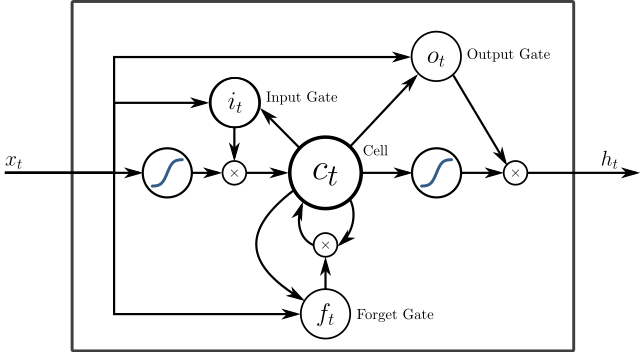
\includegraphics[width=11.5 cm]{f3.png}
\caption{Scheme of the LSTM unit.}
\label{fig3} % \label works only AFTER \caption within figure environment
\end{figure}


The LSTM-based model was used in work~\cite{DamEtAl2018} for learning both semantic and syntactic features of code. The proposed approach represents the code as a sequence of code tokens, which is fed into a LSTM system to transform code into a feature vector and a token state representing the semantic information of the token. Later the Tree-LSTM model was developed using the AST representation as input~\cite{DamEtAl2019}.

A neural bug finding technique is proposed in~\cite{HabibPradel2019}. The authors train a neural network on examples of the defective and correct code, and then use the resulting binary classifier for bug detection.
To prepare a labeled dataset, the authors use the existing static bug detection software to identify the specific kind of bugs.
The code is represented as a tokens sequence and converted to a real-value vector by using the one-hot encoding for each token.
Then, a bi-directional network with LSTM is used as model.

In \cite{ShiEtAl2020}, the authors propose a model for defect prediction on the base of AST path pair representation.
To process the code, the path in the AST is extracted as combination of symbol sequence and control sequence. These sequences are fed to a Bi-LSTM network to generate a path vector. Then, all the vectors are combined using the global attention technique to generate the vector for the entire code fragment. These final embedding representations are used for classification.


\subsection{Convolutional Neural Networks}

The Convolutional Neural Networks~\cite{Goodfellow-et-al-2016} are a type of neural network specialized for processing the data with a mesh-like structure. This network is characterized by two important features. Firstly, the local connection pattern between the units is repeated over the entire network. It allows the network to capture the short-term structural context of the source code. Secondly, the each unit have the same parameters. It allows the network to learn the information on the code element irrespective of its position in the code.
The scheme of general CNN is shown in~Fig.~\ref{fig4}.

\begin{figure}[ht] %s state preferences regarding figure placement here
% use to correct figure counter if necessary
%\renewcommand{\thefigure}{2}
\centering
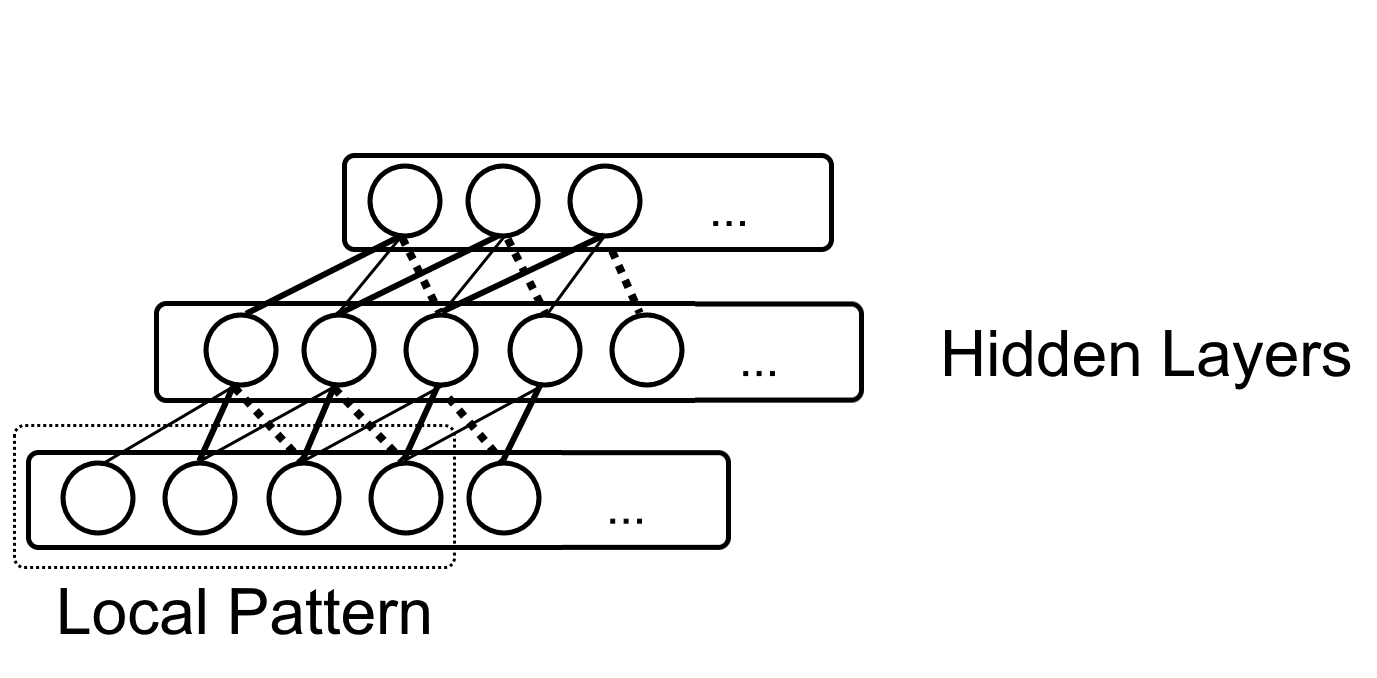
\includegraphics[width=10.5 cm]{f4.png}
\caption{Architecture of the Convolutional Neural Network.}
\label{fig4} % \label works only AFTER \caption within figure environment
\end{figure}

The work \cite{LiEtAl2017} presents the model based on the CNN architecture. Based on the program's AST, the token vectors are extracted and converted to numerical vectors. Then, these vectors are fed into a CNN. After that, the combination of the extracted semantic and structural features and code metrics is used for software defect prediction applying the logistic regression.

A deep learning model to predict defects on the basis of the commit messages and code changes is developed in work~\cite{HoangEtAl2019}. This model is based on the CNN. It uses the convolutional network layers for processing the code changes and commit text and the feature combination layer to fuse these two embedding vectors into a single one.

Another deep learning-based model for defect prediction is proposed in work~\cite{XuEtAl2019}. The training of the neural network utilizes the triplet loss technique and the weighted cross-entropy loss technique. The random forest is used as a classifier.

In \cite{QiuLuCaiJiang2019}, the features learning technique based on CNN is proposed. This model extract features from token vectors in the AST of the code and learns the transferable joint features. Combining these deep-learning-generated features with the hand-crafted ones allows the model to perform the cross-project defect prediction. Later the authors propose a new tree-based convolutional network to perform this task~\cite{CaiLuQiu2019}. It uses the tree-based continuous bag-of-word for encoding the AST nodes to be fed into CNN.

\subsection{Transformer models}

In recent time, the big success of pre-trained contextual representations in the NLP, \textit{e.g.}, \cite{liu2019roberta}, led to a rise of attempts to apply these techniques to source code. Usually, these models are based on the multi-layer Transformer architecture~\cite{vaswani2017attention} shown in Fig.~\ref{fig5}. They are pre-trained using the massive unlabeled corpora of programs with the self-supervised objectives, such as masking language modeling and next sentence prediction~\cite{KanadeEtAl2019,FengEtAl2020}. After the pre-training phase, the model can be fine-tuned for specific tasks using the supervised techniques.

\begin{figure}[ht] %s state preferences regarding figure placement here
% use to correct figure counter if necessary
%\renewcommand{\thefigure}{2}
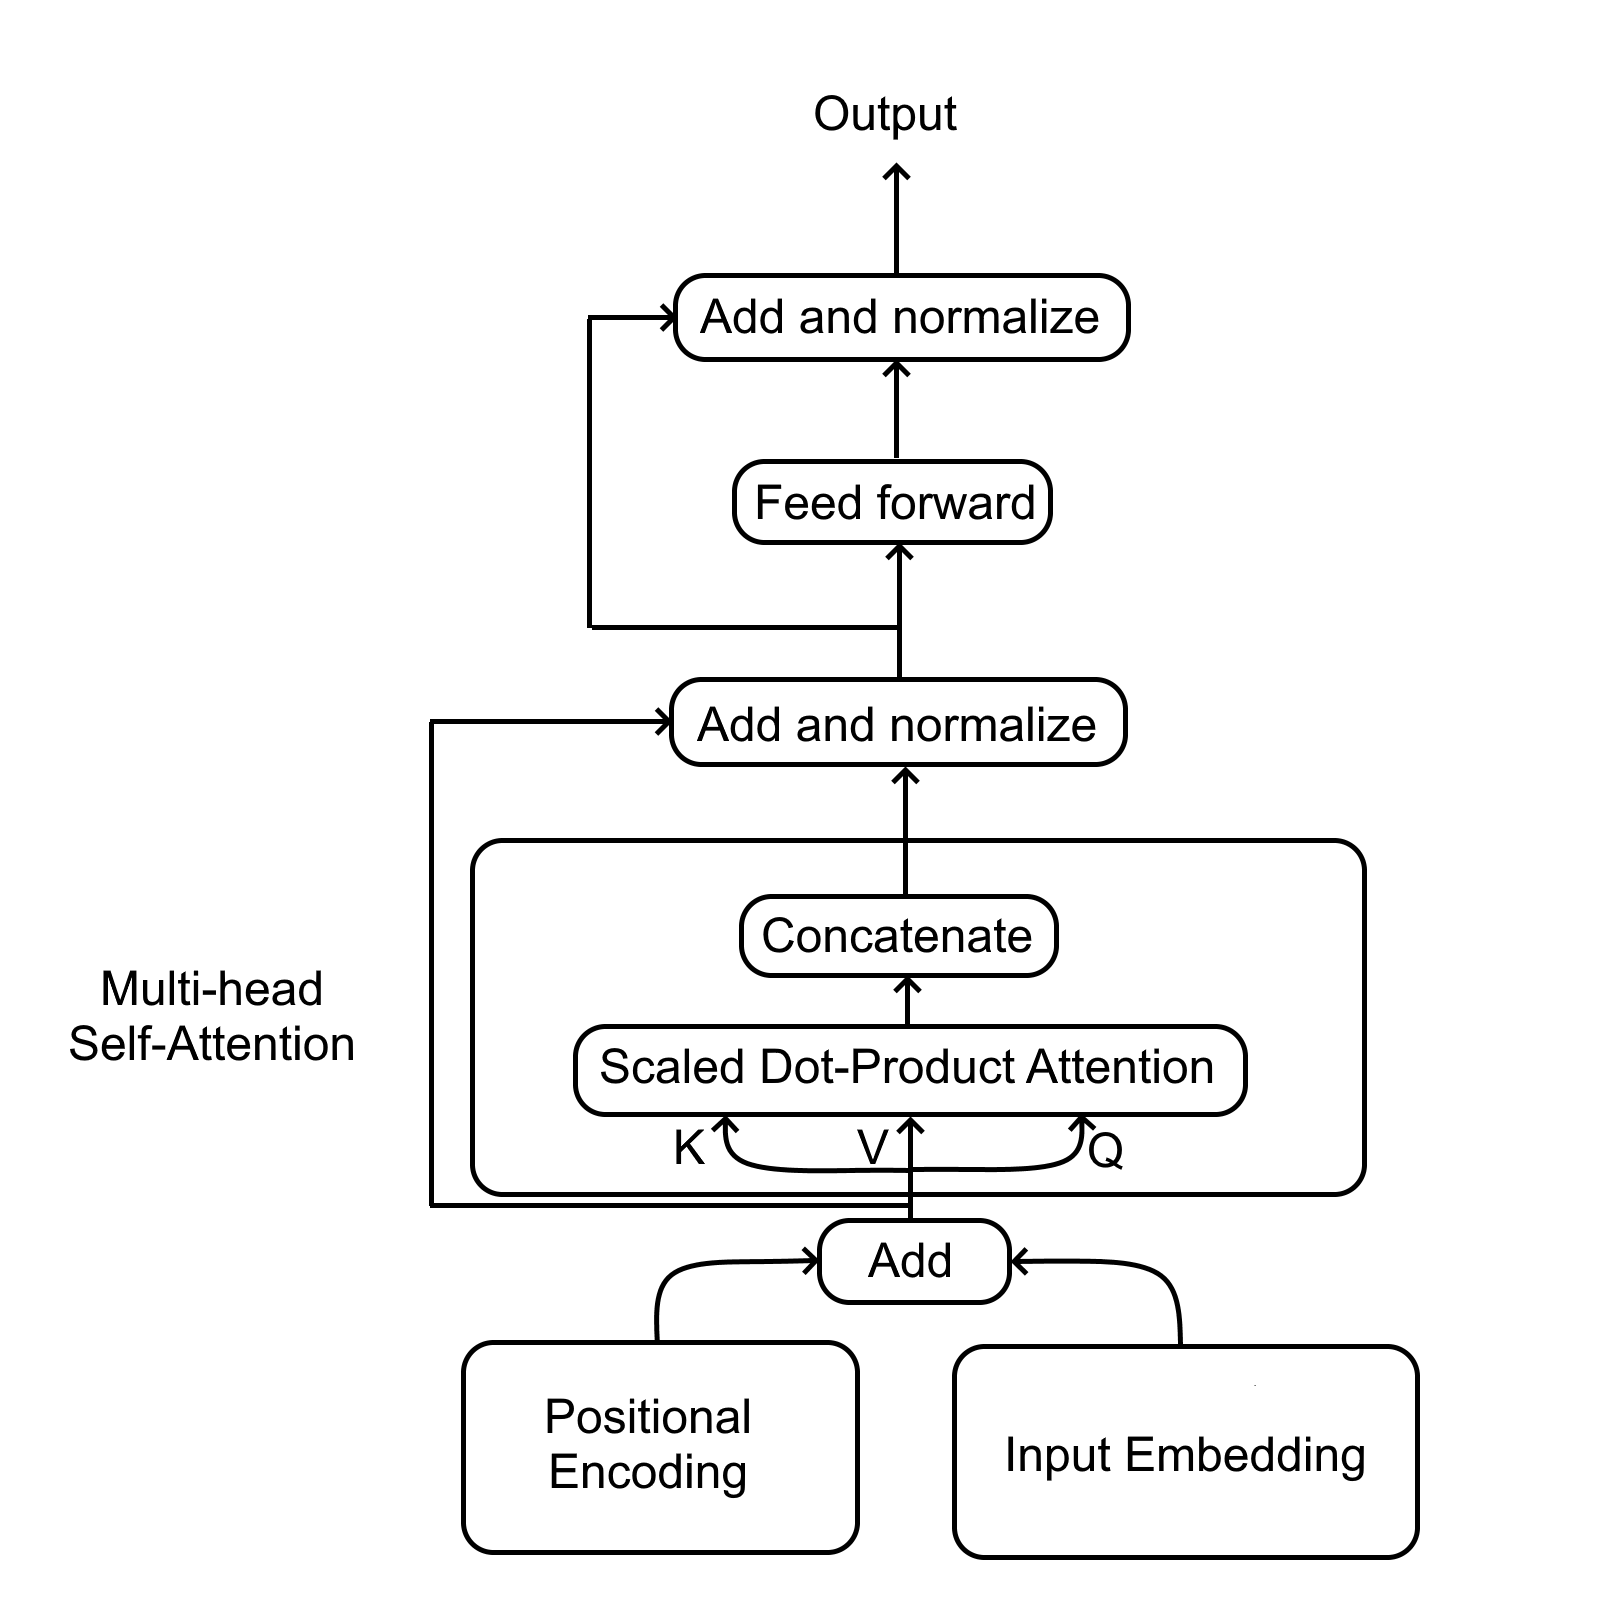
\includegraphics[width=10.5 cm]{f5.png}
\caption{Architecture of the multi-layer transformer.}
\label{fig5} % \label works only AFTER \caption within figure environment
\end{figure}

The authors of work~\cite{HumphreysDam2019} state that the approaches based on the traditional complexity metrics are useless since there is no need for a tool to tell the engineer that longer and more complex code is more defect-prone. The methods %~\cite{WangEtAl2016} 
of learning features from the source code does not guarantee capturing semantic and syntactical similarity, and very similar source code can have very different features. These features can correlate with defects rather than directly cause them.
In contrast, the authors propose the approach based on the self attention transformer encoder to the semantic defect prediction. The matrix representing the defectiveness of each token in the fragment is generated. Attention and layer normalization are used as a regularization technique. The resulting model provides the defect prediction with the semantic highlight of defective code regions.

The CuBERT model is presented in work~\cite{KanadeEtAl2019}. The authors use a corpus of Python files from the GitHub to create a benchmark for evaluating code embeddings on five classification tasks and a program repair task.
They train their model and compare it with various other models including the BiLSTM and Transformer.
It is shown that the CuBERT outperforms the baseline models consistently.

A bimodal language model called CodeBERT is presented in work~\cite{FengEtAl2020}. It is based on the multilayer bidirectional Transformer neural architecture. To prepare the data, the natural language text is represented as a sequence of words, and the source code is presented as a sequence of tokens.
The output of the CodeBERT model is a contextual vector learned from the natural language and source code, as well as, the aggregated sequence.
The resulting model efficiently solves the problems of both code to the documentation and natural language code search. 

Work~\cite{guo2021graphcodebert} presents a multi-layer bidirectional transformer architecture GraphCodeBERT, which utilizes three components as input: the source code, paired comments, and data flow graph. Data flow graph represents relations between variables, for example, where the value of a variable comes from. This allows the model to consider the code structure for code representation. For pre-training tasks, the traditional masked language modeling, as well as, the edge prediction and node alignment of data flow graph were used.
It supports several downstream code-related tasks including the code clone detection, code translation, and code refinement.


\subsection{Other Networks}

In~\cite{TongLiuWang2018}, a software defect prediction technique based on stacked denoising autoencoders model is presented. The stacked denoising autoencoder is used to extract higher-level features from the traditional metrics. The two-stage ensemble learning is used for classification. To address the class imbalance, the authors use the ensemble learning strategy. Later, the feature selection algorithm was applied to this method to address the feature renundancy problem~\cite{TranHanhBinh2019}.

A model for the software defect prediction was constructed in work~\cite{ZhaoEtAl2019} on the base of the Siamese parallel fully-connected networks. This model utilizes the paired parallel Siamese networks architecture and the deep learning approach. The network produces the high-level features that are used for classification. To address the imbalance between the minority and majority classes, the network takes into account the cost-sensitivity features.

The neural forest networks are used to learn feature representations in work~\cite{QiuEtAl2019}. To perform classification, a decision forest is used. It also guides the learning of the neural network. 
In \cite{ZhouEtAl2019}, a new deep forest model is proposed for the software defect prediction. 
To detect the essential defect features, it uses the cascade learning strategy, which consists in reforming a set of the random forest classifiers into a layered network.

The graph neural network to predict the software defects is constructed in work~\cite{XuWangAi2020}. It extracts the semantics and context features from the AST of the code fragments. To capture the defect-related information from the source code, the ASTs for the buggy and fixed version of a fragment are constructed and pruned using the community detection algorithm, which extracts the defect-related subtree.
Then, the Graph Neural Network is used to capture the latent defect information.


%%%%%%%%%%%%%%%%%%%%%%%%%%%%%%%
\section{RQ2. What are the key factors contributing to difficulty of the problem?} \label{sec_4}

The problem of software defect prediction is considered very complex and very challenging for the machine learning models based on the neural networks. 

\subsection{Lack of data}

One of the difficulties is lack of available large labeled datasets devoted to the defect prediction. To alleviate this problem, one can utilize the pre-trained contextual embeddings. This technique consists in pre-training the language model on a massive corpora of unlabeled source code using the self-supervised objectives, such as masked language modeling, next sentence prediction, and replaced token detection. 

Table~\ref{t1} presents the popular unlabeled code datasets suitable for this task.

\begin{specialtable}[H] 
\caption{List of unlabeled datasets.\label{t1}}
%%% \tablesize{} %% You can specify the fontsize here, e.g., \tablesize{\footnotesize}. If commented out \small will be used.
\renewcommand{\arraystretch}{2.0}
%\begin{tabular}{cccc}
\begin{tabulary}{.7\textwidth}{CLLLl}
\toprule
\textbf{Dataset}	& \textbf{Content}	& \textbf{Size}  & \parbox{10em}{\textbf{Used in tasks}}\\
\midrule
Bigquery github repos~\cite{kanade20cubert} & Python source code & 4M files & Pre-training CuBERT model \\
Py150~\cite{RaychevEtAl2016Deep3} & Python source code, AST & 8 423 repos, 149 993 files & Fine-tuning CuBERT model \\
%Variable-Misuse Classification, Wrong Binary Operator, Swapped Operand, Function-Docstring Mismatch, Exception Type, Variable-Misuse Localization and Repair \\
Js150~\cite{RaychevEtAl2016} & Javascript source code, AST & 150 000 source files & Code Summarization; Defect Prediction\\
Datasets for~\cite{AlonEtAl2019seq} & Java source code & 9 500 projects, 16M samples in the largest one & Code summarization \\
GitHub Java Corpus~\cite{AllamanisSutton2013} & Java source code & 11 000 projects & Language Modeling \\
CodeNN Dataset~\cite{IyerEtAl2016} & C\# source code and summaries & 66 015 fragments & Code Captioning \\
Dataset for~\cite{BryksinEtAl2020} & Kotlin source code, AST, bytecode & 47 751 repos, 932 548 files, 4 044 790 functions & Anomaly detection, defect prediction \\
Dataset for~\cite{AllamanisBrockschmidtKhademi2018} & C\# source code & 29 projects, 2.9M lines of code & Variable Misuse detection \\
\bottomrule
\end{tabulary}
\end{specialtable}

%Libraries.io & Metadata for software packages & 306k packages & Empirical Comparison of Dependency Network \\
%GHTorrent & GitHub metadata & &	\\


The pre-trained model then may be fine-tuned for the defect prediction using much smaller labeled datasets. Table~\ref{t2} presents a list of publicly available datasets devoted to the defect prediction. Usually, such datasets include pairs of correct and defective code fragments. 

\begin{specialtable}[H] 
\caption{List of labeled datasets.\label{t2}}
%%% \tablesize{} %% You can specify the fontsize here, e.g., \tablesize{\footnotesize}. If commented out \small will be used.
%\tablesize{\footnotesize}
\renewcommand{\arraystretch}{2.0}
%\begin{tabular}{cccc}
\begin{tabulary}{.7\textwidth}{CLLLl}
\toprule
\textbf{Dataset}	& \textbf{Content}	& \textbf{Size}  & \parbox{10em}{\textbf{Used in tasks}}\\
\midrule
SEIP Lab Software Defect Prediction Data~\cite{mauvsa2016systematic} & Complexity metrics & 5 subsequent releases of 3 projects from the   Java Eclipse community & Data collection and linking \\
PROMISE Software Engineering Repository~\cite{sayyad2005promise} & Numeric metrics; reported defects (false/true) & 15 000 modules & Defect prediction \\
NASA Defect Dataset~\cite{shepperd2018nasa} & Numeric metrics; reported defects (false/true) & 51 000 modules & Defect prediction \\
REPD datasets~\cite{AfricEtAl2020} & Numeric metrics, semantic features, reported defects & 10885 fragments in the largest one & Defect prediction \\
GPHR~\cite{ghpr2020} & Java code and metrics & 3526 pairs of fragments, buggy and fixed, code metrics & Defect prediction \\
BugHunter\cite{FerencEtAl2020} & Java source code; metrics; fix-inducing commit; number of reported bugs & 159k pairs for 3 granularity levels (file/class/method), 15 projects & Analyzing the importance of complexity   metrics \\
GitHub Bug DataSet~\cite{ferenc2016github_bug} & Java source code; code metrics; number of reported bugs and vulnerabilities & 15 projects; 183k classes & Bug prediction \\
Unified Bug Dataset~\cite{ferenc2020public} & Java source code; code metrics; number of reported bugs & 47 618 classes; 43 744 files & Bug prediction \\
Neural Code Translator Dataset~\cite{TufanoEtAl2018} & Pairs of buggy and fixed abstracted method-level fragments & 46k pairs of small fragments (under 50 tokens), 50k pairs of medium fragments (under 100 tokens) & Code refinement \\
BugsInPy~\cite{WidyasariEtAl2020} & Pair of buggy and fixed Python snippets, manually processed & 493 bugs from 17 projects & Benchmark for testing and debugging tools \\
\bottomrule
\end{tabulary}
\end{specialtable}


\begin{specialtable}[H] 
%\caption{List of labeled datasets.}
%%% \tablesize{} %% You can specify the fontsize here, e.g., \tablesize{\footnotesize}. If commented out \small will be used.
%\tablesize{\footnotesize}
\renewcommand{\arraystretch}{2.0}
%\begin{tabular}{cccc}
\begin{tabulary}{.7\textwidth}{CLLLl}
\toprule
\textbf{Dataset}	& \textbf{Content}	& \textbf{Size}  & \parbox{10em}{\textbf{Used in tasks}}\\
\midrule
Draper VDISC Dataset~\cite{RusselEtAl2018} & C and C++ source code, labeled for potential vulnerabilities & 1.27M functions & Vulnerability Detection \\
Refactory Dataset~\cite{yang2019refactory} & Python source code & 2 442 correct and 1 783 buggy program & Program repair \\
\hbox{Defect4J}\cite{just2014defects4j} & Java source code & 835 pairs of buggy and fixed fragments & Software testing research \\
BugSwarm\cite{Tomassi2019bugswarm} & Java and Python source code & 3 232 pairs of buggy and fixed fragments & Software testing research \\
BuGL~\cite{muvva2020bugl} & C, C++, Java, and Python source code; issues; pull requests & 54 projects; 151k closed issues; 10 187 pull requests & Bug localization \\
Bugs.jar~\cite{SahaEtAl2018bugsjar} & Java source code & 1 158 pairs of buggy and and fixed fragments & Program repair \\
\bottomrule
\end{tabulary}
\end{specialtable}

As the other factors affecting the difficuty of constructing datasets, we can highlight that the distribution of the classes in the real code projects is often imbalanced. Usually, there are fewer buggy files or methods in a project than the correct ones. This may lead to the situation where the common classifiers would correctly detect the major class (correct code) and ignore the much smaller class of the defect-prone code.
This will lead to bad performance of the model.

To address this imbalance, several oversampling methods are proposed. In works~\cite{AlsawalqahEtAl2017,AgrawalMenzies2018}, the authors constructed hybrid approaches. It is based on the Synthetic Minority Over-Sampling Technique (SMOTE and SMOTUNED) for preparing the datasets and ensemble approaches for classifying the defective and correct code.
In \cite{ShiEtAl2020}, the authors takes into account the proportion of the correct and defective code in each project in the dataset. To balance the classes, they duplicate the elements of the smaller class.

\subsection{Lack of context}

Another problem is the complexity of the context for the code. Unlike the natural texts, the code element may depend on another element located far away, maybe, even in another code fragment. Moreover, it is often hard to say if the code element is defective without considering its context. If dataset consists of the pairs of bugged and fixed code fragments, it is often hard to extract the essence of defect.

Approaches based on the Transformer networks were aimed to NLP problems where data display a great deal of locality of reference. Most information about a token can be derived from its neighboring tokens~\cite{ tay2020efficient}. Thus, most of such models represent the source code as a sequence of tokens.

The traditional Transformer architectures based on self-attention matrices do not scale well because of quadratic complexity. Usually, they are designed to handle the input sequences with limited length (usually, 512 or 1024 tokens)~\cite{tay2020efficient, tay2020long}.
 Therefore, their applicability to understand the context of the source code is limited.
 
There are several modifications to the Transformer architecture that improve its ability to comprehend long sequences~\cite{zaheer2021big,fiok2021text,beltagy2020longformer}. These approaches alleviate the problem of limited length of the input, giving the Transformers a potential to work with a complex context of the source code. 
 
 Another approach is to capture the structural and global relations on the code, combining the sequence-based and graph-based models for code representation~\cite{hellendoorn2020global,guo2021graphcodebert}. 

Thus, representing the code context is essential in the software defect prediction. 

%%%%%%%%%%%%%%%%%%%%%%%%%%%%%%%
\section{RQ3. What are the trends in the primary studies on the use of deep learning for the software defect prediction?} \label{sec_5}

Earliest works such as~\cite{YangEtAl2015} utilize the deep learning techniques trying to extract the implicit features from the traditional explicit features (such as code metrics).
The main drawback of this approach is that these traditional features usually cannot capture the semantic difference between the correct and defective code. Therefore, the combination of these features would also fail to do this~\cite{LiEtAl2017}.

Later approaches~\cite{DamEtAl2019,HoangEtAl2019} use the generic or tailored deep learning techniques to extract the semantic and syntactic features directly from the source code, usually, from the abstract syntax trees. These deep learned features are used in combination with the traditional ones in the machine classifiers to produce the accurate defect prediction.

Modern software development often prioritize writing the human-readable source code. This includes using the  meaningful names for the functions and variables and writing the code documentation in natural language. This leads to the situation where we can extract the semantic information from the source code using the techniques originally intended for the NLP, such as the pre-trained language representations such as BERT~\cite{devlin2019bert}. 

Learning useful models with supervised setting is often difficult because labeled data are usually limited. Thus, many unsupervised approaches have been proposed recently to utilize the large unlabeled datasets that are more readily available. Usually, this means that pre-training is performed with automatic supervisions without manual annotation of the samples. Then, the model may be fine-tuned for the specific task using much smaller supervised data~\cite{kanade20cubert}.

The most recent techniques in software engineering are based on using the general-purposed pre-trained models for programming languages~\cite{karampatsis2020scelmo,guo2021graphcodebert}. These models learn to ``understand'' the source code from unlabeled datasets using the self-supervised objectives. Large corpus of source code is used for pre-training. Usually, the objective is the Masked Language Modeling where at some positions the tokens are masked out and the model must predict the original token~\cite{FengEtAl2020}. 
Utilizing these techniques alleviates the need for the task-specific architectures and training on large labeled datasets for each task separately.


%%%%%%%%%%%%%%%%%%%%%%%%%%%%%%%%%%%%%%%%%%
\section{Conclusions} \label{sec_6}

One of the major challenges in the modern software engineering is predicting defective code. Recent developments in the field of machine learning, especially the multi-layered neural networks and deep learning algorithms, provide powerful techniques, which utilize learning algorithms for representations of the source code that captures the semantic and structural information. 

This survey presents the latest research progress in software defect prediction using the deep learning techniques, such as the Transformer architectures. We formulate the main difficulties of the defect prediction problem as lack of data and complexity of context and discuss the ways to alleviate these problems.

Taking into account the latest trends in the machine learning techniques for the software defect prediction problem, we believe that progress in this field will be achieved largely due to the implementation of the following ideas.
\begin{itemize}
\item To reduce the requirements for the size of the labeled datasets, one should use the self-supervised training on large corpora of the unlabeled data. In addition, it is necessary to use the unlabeled data for the pre-training of related tasks and to contribute to the fact that the trained models will have a deeper and more comprehensive understanding of the source code. This, in the turn, will allow one to find the deeper defects.
\item To leverage the latest advances in the machine learning techniques in the natural language processing in the programming languages, we are already seeing the successful migration of these methods to solve various code understanding problems. For example, optimization of the self-attention mechanism for the transformers will allow one to use them for long sequences, which, in the turn, will lead to a more complete consideration of the code context for finding the defects.
\item Often a defect is not limited to a single line of code or one function, and there are various ways to fix it. For example, a bug can be fixed either inside the function or at calling this function. Thus, the defect ceases to have specific coordinates inside the source file. In addition, not being an explicit defect, a line of code can become defective at a certain point in time. A changed context may lead to the fact that the purpose of the code changes, and, therefore, the old implementation no longer corresponds to the new requirements or specifications. 
\end{itemize}

All this leads to a blurring of the concept of a defect. Thus, we come to the concepts of ``potentially defective'' code or ``strange'' code. In this regard, as promising problems, we want to note the task of finding an atypical (or anomalous) code and the task of the code refinement. These task require good representations of the code and code changes, taking into account the specifics of the source code, such as structure and context.

It is difficult to state which of the state-of-the-art models performs in the best way. There are no universally accepted standard benchmarks for the problem and different researchers utilize different performance metrics and use different data. Thus, the experimental results from the primary works cannot be directly compared. The existing comparative studies such as~\cite{Herbold2018benchmark} show that while the state-of-the-art deep learning techniques usually perform better than standard deep learning and traditional metrics-based ones (achieving the increase of F1 from 60\% up to 80\% in some cases). None of the approaches achieves a consistently high performance in terms of recall, precision, and accuracy sufficient for the practical application. Thus, the defect prediction problem remains an open one.

%%%%%%%%%%%%%%%%%%%%%%%%%%%%%%%%%%%%%%%%%%
%\section{Patents}

%This section is not mandatory, but may be added if there are patents resulting from the work reported in %this manuscript.

%%%%%%%%%%%%%%%%%%%%%%%%%%%%%%%%%%%%%%%%%%
\vspace{6pt} 

%%%%%%%%%%%%%%%%%%%%%%%%%%%%%%%%%%%%%%%%%%
%% optional
%\supplementary{The following are available online at \linksupplementary{s1}, Figure S1: title, Table S1: title, Video S1: title.}

% Only for the journal Methods and Protocols:
% If you wish to submit a video article, please do so with any other supplementary material.
% \supplementary{The following are available at \linksupplementary{s1}, Figure S1: title, Table S1: title, Video S1: title. A supporting video article is available at doi: link.} 

%%%%%%%%%%%%%%%%%%%%%%%%%%%%%%%%%%%%%%%%%%
\authorcontributions{All authors (E.N.A., A.Yu.B., A.A.D., K.S.K., A.V.K., I.P.M., V.E.M.) contributed equally. All authors have read and agreed to the published version of the manuscript.}
%{For research articles with several authors, a short paragraph specifying their individual contributions must be provided. The following statements should be used ``Conceptualization, X.X. and Y.Y.; methodology, X.X.; software, X.X.; validation, X.X., Y.Y. and Z.Z.; formal analysis, X.X.; investigation, X.X.; resources, X.X.; data curation, X.X.; writing---original draft preparation, X.X.; writing---review and editing, X.X.; visualization, X.X.; supervision, X.X.; project administration, X.X.; funding acquisition, Y.Y. All authors have read and agreed to the published version of the manuscript.'', please turn to the  \href{http://img.mdpi.org/data/contributor-role-instruction.pdf}{CRediT taxonomy} for the term explanation. Authorship must be limited to those who have contributed substantially to the work~reported.}

\funding{This research received no external funding.}
%{Please add: ``This research received no external funding'' or ``This research was funded by NAME OF FUNDER grant number XXX.'' and  and ``The APC was funded by XXX''. Check carefully that the details given are accurate and use the standard spelling of funding agency names at \url{https://search.crossref.org/funding}, any errors may affect your future funding.}

%\institutionalreview{In this section, please add the Institutional Review Board Statement and approval number for studies involving humans or animals. Please note that the Editorial Office might ask you for further information. Please add ``The study was conducted according to the guidelines of the Declaration of Helsinki, and approved by the Institutional Review Board (or Ethics Committee) of NAME OF INSTITUTE (protocol code XXX and date of approval).'' OR ``Ethical review and approval were waived for this study, due to REASON (please provide a detailed justification).'' OR ``Not applicable'' for studies not involving humans or animals. You might also choose to exclude this statement if the study did not involve humans or animals.}

%\informedconsent{Any research article describing a study involving humans should contain this statement. Please add ``Informed consent was obtained from all subjects involved in the study.'' OR ``Patient consent was waived due to REASON (please provide a detailed justification).'' OR ``Not applicable'' for studies not involving humans. You might also choose to exclude this statement if the study did not involve humans.

%Written informed consent for publication must be obtained from participating patients who can be identified (including by the patients themselves). Please state ``Written informed consent has been obtained from the patient(s) to publish this paper'' if applicable.}

%\dataavailability{In this section, please provide details regarding where data supporting reported results can be found, including links to publicly archived datasets analyzed or generated during the study. Please refer to suggested Data Availability Statements in section ``MDPI Research Data Policies'' at \url{https://www.mdpi.com/ethics}. You might choose to exclude this statement if the study did not report any data.} 

%\acknowledgments{In this section you can acknowledge any support given which is not covered by the author contribution or funding sections. This may include administrative and technical support, or donations in kind (e.g., materials used for experiments).}

\conflictsofinterest{The authors declare no conflict of interest. }

%{Declare conflicts of interest or state ``The authors declare no conflict of interest.'' Authors must identify and declare any personal circumstances or interest that may be perceived as inappropriately influencing the representation or interpretation of reported research results. Any role of the funders in the design of the study; in the collection, analyses or interpretation of data; in the writing of the manuscript, or in the decision to publish the results must be declared in this section. If there is no role, please state ``The funders had no role in the design of the study; in the collection, analyses, or interpretation of data; in the writing of the manuscript, or in the decision to publish the~results''.} 

%% Optional
%\sampleavailability{Samples of the compounds ... are available from the authors.}

%%%%%%%%%%%%%%%%%%%%%%%%%%%%%%%%%%%%%%%%%%
%% Only for journal Encyclopedia
%\entrylink{The Link to this entry published on the encyclopedia platform.}

%%%%%%%%%%%%%%%%%%%%%%%%%%%%%%%%%%%%%%%%%%
%% Optional
\abbreviations{Abbreviations}{
The following abbreviations are used in this manuscript:\\

\noindent 
\begin{tabular}{@{}ll}
AST & Abstract Syntax Tree\\
CNN & Convolutional Neural Network\\
DBN & Deep Belief Network\\
DL & Deep Learning\\
LSTM & Long Short Term Memory\\
%ML & Machine Learning\\
NLP & Natural Language Processing\\
SDP & Software Defect Prediction\\
\end{tabular}}

%%%%%%%%%%%%%%%%%%%%%%%%%%%%%%%%%%%%%%%%%%
\end{paracol}
%%%%%%%%%%%%%%%%%%%%%%%%%%%%%%%%%%%%%%%%%%
\reftitle{References}

% Please provide either the correct journal abbreviation (e.g. according to the “List of Title Word Abbreviations” http://www.issn.org/services/online-services/access-to-the-ltwa/) or the full name of the journal.
% Citations and References in Supplementary files are permitted provided that they also appear in the reference list here. 

%=====================================
% References, variant A: external bibliography
%=====================================
\externalbibliography{yes}
\bibliography{references}

% If authors have biography, please use the format below
%\section*{Short Biography of Authors}
%\bio
%{\raisebox{-0.35cm}{\includegraphics[width=3.5cm,height=5.3cm,clip,keepaspectratio]{Definitions/author1.pdf}}}
%{\textbf{Firstname Lastname} Biography of first author}
%
%\bio
%{\raisebox{-0.35cm}{\includegraphics[width=3.5cm,height=5.3cm,clip,keepaspectratio]{Definitions/author2.jpg}}}
%{\textbf{Firstname Lastname} Biography of second author}

% The following MDPI journals use author-date citation: Arts, Econometrics, Economies, Genealogy, Humanities, IJFS, JRFM, Laws, Religions, Risks, Social Sciences. For those journals, please follow the formatting guidelines on http://www.mdpi.com/authors/references
% To cite two works by the same author: \citeauthor{ref-journal-1a} (\citeyear{ref-journal-1a}, \citeyear{ref-journal-1b}). This produces: Whittaker (1967, 1975)
% To cite two works by the same author with specific pages: \citeauthor{ref-journal-3a} (\citeyear{ref-journal-3a}, p. 328; \citeyear{ref-journal-3b}, p.475). This produces: Wong (1999, p. 328; 2000, p. 475)

%%%%%%%%%%%%%%%%%%%%%%%%%%%%%%%%%%%%%%%%%%
%% for journal Sci
%\reviewreports{\\
%Reviewer 1 comments and authors’ response\\
%Reviewer 2 comments and authors’ response\\
%Reviewer 3 comments and authors’ response
%}
%%%%%%%%%%%%%%%%%%%%%%%%%%%%%%%%%%%%%%%%%%
\end{document}

